\section{Hardware components}
\label{sec:hardwareComponents}
In the very beginning of the project, the team looked into the possibility of getting live data directly from devices. This required some technical equipment for collecting and transmitting power usage from a device. The original idea was that the app should get data directly from devices in the house, and if possible, control the devices.

The team concluded that the only reasonable architecture for a such a system would include a small server, running on a small computer (for example Raspberry Pi), and measurement devices with a wireless transmitter connected to anything the user wanted to control and monitor. Finding already usable devices that allow for energy monitoring on the market was not achieved with much success. Communication between the home server and devices is also a challenge. Much of this is due to the lack of standards in transmission between devices and servers. The technology on this front is currently moving very fast due to the ongoing \gls{IoT} trend. The team found that many of the existing apps would have a device that were desired, but with a proprietary communication protocol and technology. The customer had previously requested that the devices should be cheap and preferably based on open source technology.

\subsection{Home data aggregator}
To ensure full operability 24 hours a day, a base station is needed in the user's home. This server will serve as an aggregating agent for data from measuring units attached to devices. Given an ideal architecture implementation, this unit would also be responsible for controlling devices. The team envisions this unit as a synchronization service working for the Wattitude cloud server. The software for such a server could be based on the current server software made. The hardware for this base station would be as simple as a Raspberry pi~\cite{pi}. These computers are small, cheap and provides all the hardware needed for a simple home aggregator. Some modifications might be necessary to communicate with the measuring units. The architecture for this aggregation unit is shown in figure~\ref{fig:aggregator}.

\begin{figure}[H]
\centering
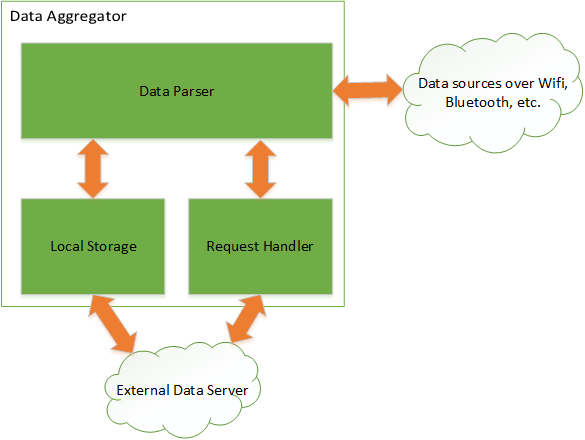
\includegraphics[height=0.4\textheight]{ch/further/fig/home.png}
\caption{Detailed architecture for the home data aggregator}
\label{fig:aggregator}
\end{figure}

\subsection{Measuring unit}
To make real time monitoring possible, every device the user wants to monitor must be connected to a wireless monitoring unit. The team tried to find an existing solution that was satisfying, but most of the options found was proprietary and/or to expensive. The following paragraphs describes the most viable options.

\subsubsection{HomeMatic plug}
This is the device that the CoSSMic team at SINTEF has been experimenting with. The drawbacks is that it has a unit price of almost 500 NOK and must be imported. Covering most home devices with such a measuring device would be extremely costly. It is part of the HomeMatic proprietary hardware line, and is meant to interface with a HomeMatic central control unit, much like the base station described above. As hardware devices were not a part of the project scope, the team did not do any research on how to interface with this unit. %The only knowledge we have is that the SINTEF team working on CoSSMic has been working on it.

\subsubsection{Do It Yourself (DIY) Arduino}
A much cheaper, but perhaps limited solution, is one from Open Energy Monitor~\cite{oemmodule}. These units do not support the ability to control devices, only measurement of consumption. They are much cheaper than the HomeMatic unit, but must be assembled manually. The unit can be good for experimenting and prototyping but it is far from ready for the home market.
